\chapter{SOURCE CODE AND NOTEBOOKS 
\label{appendix:source_code}}

To facilitate reproducibility and foster further research, the complete source code and Jupyter notebooks employed in this dissertation have been made publicly available on GitHub. This repository encompasses all scripts, codes, and supplementary materials essential for replicating the experiments and analyses presented herein. By providing access to these resources, we aim to promote transparency and encourage collaboration within the research community. The repository can be accessed at the link below, where detailed instructions for usage and setup are also provided in a README.md file (Figure \ref{fig:source_code_at_github}). 

\vspace{1cm}

\href{https://github.com/alf2001br/Master_thesis_Andre_Luiz_Florentino_project/tree/main}{https://github.com/alf2001br/Master\_thesis\_Andre\_Luiz\_Florentino\_project/tree/main}

\vspace{1cm}


\begin{figure}[htbp]
    \raggedright
        \caption{README file of the GitHub project.}
        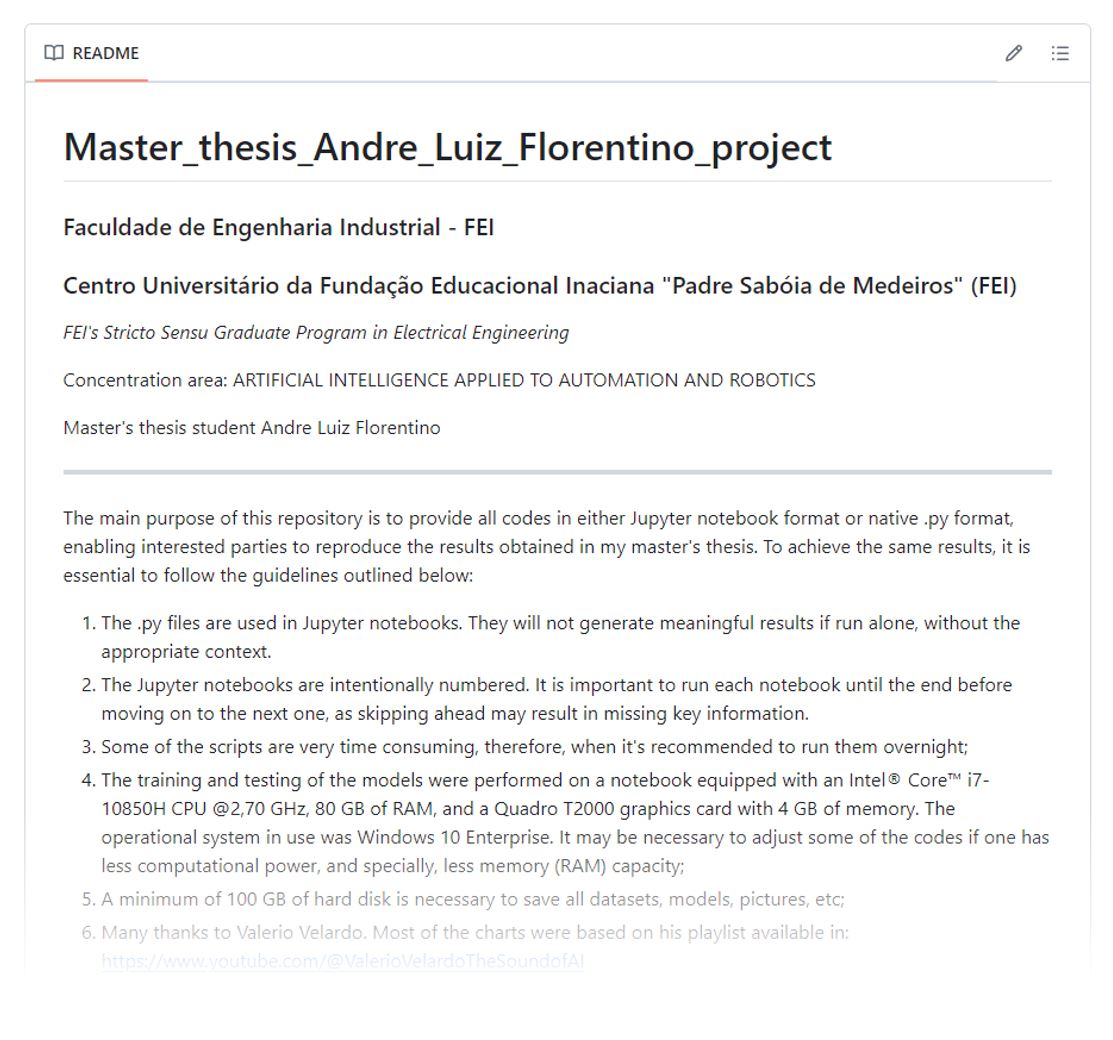
\includegraphics[width=0.80\textwidth]{resources/images/090-source_code/GitHub_project.jpg}
        \smallcaption{Source: Author}
        \label{fig:source_code_at_github}
\end{figure}
